% Created by tikzDevice version 0.11 on 2018-09-26 18:45:55
% !TEX encoding = UTF-8 Unicode
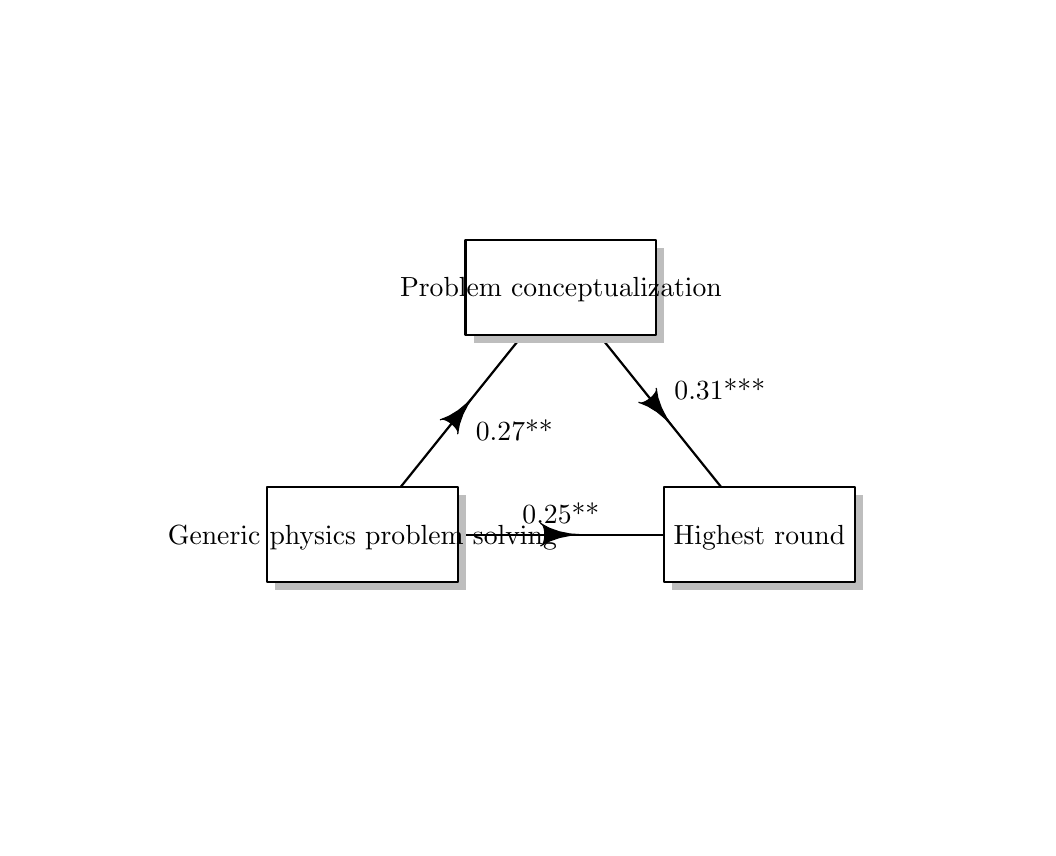
\begin{tikzpicture}[x=1pt,y=1pt]
\definecolor{fillColor}{RGB}{255,255,255}
\path[use as bounding box,fill=fillColor,fill opacity=0.00] (0,0) rectangle (361.35,289.08);
\begin{scope}
\path[clip] ( 49.20, 61.20) rectangle (336.15,239.88);
\definecolor{drawColor}{RGB}{0,0,0}

\path[draw=drawColor,line width= 0.8pt,line join=round,line cap=round] (192.68,195.21) -- (264.41,105.87);

\path[draw=drawColor,line width= 0.4pt,line join=round,line cap=round] (227.83,151.43) -- (228.54,150.54);
\definecolor{fillColor}{RGB}{0,0,0}

\path[draw=drawColor,line width= 0.4pt,line join=round,line cap=round,fill=fillColor] (227.10,158.77) --
	(227.73,155.25) --
	(228.98,151.67) --
	(230.80,148.15) --
	(233.13,144.83) --
	(233.13,144.83) --
	(230.39,147.82) --
	(227.35,150.36) --
	(224.12,152.35) --
	(220.82,153.73) --
	(220.82,153.73) --
	(221.11,153.53) --
	(221.54,153.47) --
	(222.10,153.54) --
	(222.74,153.75) --
	(223.45,154.09) --
	(224.19,154.54) --
	(224.91,155.07) --
	(225.58,155.66) --
	(226.18,156.28) --
	(226.66,156.90) --
	(227.00,157.48) --
	(227.20,158.01) --
	(227.23,158.44) --
	(227.10,158.77) --
	cycle;

\node[text=drawColor,anchor=base west,inner sep=0pt, outer sep=0pt, scale=  1.00] at (233.71,154.73) { 0.31*** };

\path[draw=drawColor,line width= 0.8pt,line join=round,line cap=round] (120.94,105.87) -- (192.68,195.21);

\path[draw=drawColor,line width= 0.4pt,line join=round,line cap=round] (156.09,149.65) -- (156.81,150.54);

\path[draw=drawColor,line width= 0.4pt,line join=round,line cap=round,fill=fillColor] (149.08,147.35) --
	(152.38,148.73) --
	(155.61,150.72) --
	(158.66,153.26) --
	(161.39,156.25) --
	(161.39,156.25) --
	(159.07,152.93) --
	(157.24,149.41) --
	(155.99,145.83) --
	(155.36,142.31) --
	(155.36,142.31) --
	(155.49,142.64) --
	(155.46,143.07) --
	(155.27,143.60) --
	(154.92,144.18) --
	(154.44,144.80) --
	(153.85,145.42) --
	(153.17,146.01) --
	(152.45,146.54) --
	(151.71,146.99) --
	(151.01,147.33) --
	(150.36,147.54) --
	(149.81,147.61) --
	(149.37,147.55) --
	(149.08,147.35) --
	cycle;

\node[text=drawColor,anchor=base west,inner sep=0pt, outer sep=0pt, scale=  1.00] at (161.97,139.83) { 0.27** };

\path[draw=drawColor,line width= 0.8pt,line join=round,line cap=round] (120.94,105.87) -- (264.41,105.87);

\path[draw=drawColor,line width= 0.4pt,line join=round,line cap=round] (191.24,105.87) -- (192.68,105.87);

\path[draw=drawColor,line width= 0.4pt,line join=round,line cap=round,fill=fillColor] (185.35,109.90) --
	(188.49,108.19) --
	(192.07,106.92) --
	(195.96,106.13) --
	(200.00,105.87) --
	(200.00,105.87) --
	(195.96,105.61) --
	(192.07,104.82) --
	(188.49,103.55) --
	(185.35,101.84) --
	(185.35,101.84) --
	(185.69,101.95) --
	(186.01,102.24) --
	(186.30,102.72) --
	(186.54,103.36) --
	(186.72,104.12) --
	(186.83,104.97) --
	(186.87,105.87) --
	(186.83,106.77) --
	(186.72,107.62) --
	(186.54,108.38) --
	(186.30,109.02) --
	(186.01,109.50) --
	(185.69,109.79) --
	(185.35,109.90) --
	cycle;

\node[text=drawColor,anchor=base west,inner sep=0pt, outer sep=0pt, scale=  1.00] at (178.79,110.06) { 0.25** };
\definecolor{fillColor}{RGB}{190,190,190}

\path[fill=fillColor] (161.11,175.12) --
	(161.11,209.56) --
	(229.98,209.56) --
	(229.98,175.12) --
	cycle;
\definecolor{fillColor}{RGB}{255,255,255}

\path[draw=drawColor,line width= 0.8pt,line join=round,line cap=round,fill=fillColor] (158.24,177.99) --
	(158.24,212.43) --
	(227.11,212.43) --
	(227.11,177.99) --
	cycle;

\node[text=drawColor,anchor=base,inner sep=0pt, outer sep=0pt, scale=  1.00] at (192.68,191.77) {Problem conceptualization};
\definecolor{fillColor}{RGB}{190,190,190}

\path[fill=fillColor] ( 89.37, 85.78) --
	( 89.37,120.22) --
	(158.24,120.22) --
	(158.24, 85.78) --
	cycle;
\definecolor{fillColor}{RGB}{255,255,255}

\path[draw=drawColor,line width= 0.8pt,line join=round,line cap=round,fill=fillColor] ( 86.50, 88.65) --
	( 86.50,123.09) --
	(155.37,123.09) --
	(155.37, 88.65) --
	cycle;

\node[text=drawColor,anchor=base,inner sep=0pt, outer sep=0pt, scale=  1.00] at (120.94,102.43) {Generic physics problem solving};
\definecolor{fillColor}{RGB}{190,190,190}

\path[fill=fillColor] (232.85, 85.78) --
	(232.85,120.22) --
	(301.72,120.22) --
	(301.72, 85.78) --
	cycle;
\definecolor{fillColor}{RGB}{255,255,255}

\path[draw=drawColor,line width= 0.8pt,line join=round,line cap=round,fill=fillColor] (229.98, 88.65) --
	(229.98,123.09) --
	(298.85,123.09) --
	(298.85, 88.65) --
	cycle;

\node[text=drawColor,anchor=base,inner sep=0pt, outer sep=0pt, scale=  1.00] at (264.41,102.43) {Highest round};
\end{scope}
\end{tikzpicture}
